%  LaTeX support: latex@mdpi.com 
%  In case you need support, please attach all files that are necessary for compiling as well as the log file, and specify the details of your LaTeX setup (which operating system and LaTeX version / tools you are using).

% You need to save the "mdpi.cls" and "mdpi.bst" files into the same folder as this template file.

%=================================================================
\documentclass[entropy,article,submit,moreauthors,pdftex,10pt,a4paper]{mdpi} 

%
%--------------------
% Class Options:
%--------------------
% journal
%----------
% Choose between the following MDPI journals:
% actuators, admsci, aerospace, agriculture, agronomy, algorithms, animals, antibiotics, antibodies, antioxidants, applsci, arts, atmosphere, atoms, axioms, batteries, behavsci, beverages, bioengineering, biology, biomedicines, biomimetics, biomolecules, biosensors, brainsci, buildings, carbon, cancers, catalysts, cells, challenges, chemosensors, children, chromatography, climate, coatings, computation, computers, condensedmatter, cosmetics, cryptography, crystals, data, dentistry, designs, diagnostics, diseases, diversity, econometrics, economies, education, electronics, energies, entropy, environments, epigenomes, fermentation, fibers, fishes, fluids, foods, forests, futureinternet, galaxies, games, gels, genealogy, genes, geosciences, geriatrics, healthcare, horticulturae, humanities, hydrology, informatics, information, infrastructures, inorganics, insects, instruments, ijerph, ijfs, ijms, ijgi, ijtpp, inventions, jcdd, jcm, jdb, jfb, jfmk, jimaging, jof, jintelligence, jlpea, jmse, jpm, jrfm, jsan, land, languages, laws, life, literature, lubricants, machines, magnetochemistry, marinedrugs, materials, mathematics, mca, mti, medsci, medicines, membranes, metabolites, metals, microarrays, micromachines, microorganisms, minerals, molbank, molecules, mps, nanomaterials, ncrna, neonatalscreening, nutrients, particles, pathogens, pharmaceuticals, pharmaceutics, pharmacy, philosophies, photonics, plants, polymers, processes, proteomes, publications, recycling, religions, remotesensing, resources, risks, robotics, safety, sensors, separations, sexes, sinusitis, socsci, societies, soils, sports, standards, sustainability, symmetry, systems, technologies, toxics, toxins, tropicalmed, universe, urbansci, vaccines, vetsci, viruses, water
%---------
% article
%---------
% The default type of manuscript is article, but can be replaced by: 
% addendum, article, book, bookreview, briefreport, casereport, changes, comment, commentary, communication, conceptpaper, correction, conferenceproceedings, conferencereport, expressionofconcern, meetingreport, creative, datadescriptor, discussion, editorial, essay, erratum, hypothesis, interestingimage, letter, newbookreceived, opinion, obituary, projectreport, reply, retraction, review, preprints, shortnote, supfile, technicalnote
% supfile = supplementary materials
%----------
% submit
%----------
% The class option "submit" will be changed to "accept" by the Editorial Office when the paper is accepted. This will only make changes to the frontpage (e.g. the logo of the journal will get visible), the headings, and the copyright information. Also, line numbering will be removed. Journal info and pagination for accepted papers will also be assigned by the Editorial Office.
%------------------
% moreauthors
%------------------
% If there is only one author the class option oneauthor should be used. Otherwise use the class option moreauthors.
%---------
% pdftex
%---------
% The option pdftex is for use with pdfLaTeX. If eps figure are used, remove the option pdftex and use LaTeX and dvi2pdf.

%=================================================================
\firstpage{1} 
\makeatletter 
\setcounter{page}{\@firstpage} 
\makeatother 
\articlenumber{x}
\doinum{10.3390/------}
\pubvolume{xx}
\pubyear{2016}
\copyrightyear{2016}
\externaleditor{Academic Editor: name}
\history{Received: date; Accepted: date; Published: date}

%------------------------------------------------------------------
% The following line should be uncommented if the LaTeX file is uploaded to arXiv.org
%\pdfoutput=1

%=================================================================
% Add packages and commands here. The following packages are loaded in our class file: fontenc, calc, indentfirst, fancyhdr, graphicx, lastpage, ifthen, lineno, float, amsmath, setspace, enumitem, mathpazo, booktabs, titlesec, etoolbox, amsthm, hyphenat, natbib, hyperref, footmisc, geometry, caption, url, mdframed

%=================================================================
%% Please use the following mathematics environments: Theorem, Lemma, Corollary, Proposition, Characterization, Property, Problem, Example, ExamplesandDefinitions, Remark, Definition
%% For proofs, please use the proof environment (the amsthm package is loaded by the MDPI class).

%=================================================================
% Full title of the paper (Capitalized)
\Title{EEG characterization and classification based on histograms of image gradients}

% Authors, for the paper (add full first names)
\Author{Rodrigo Ramele $^{1,\dagger}$, Ana Julia Villar $^{1}$ and Juan Miguel Santos  $^{1}$*}
% Authors, for metadata in PDF
\AuthorNames{Rodrigo Ramele, Ana Julia Villar and Juan Miguel Santos}

% Affiliations / Addresses (Add [1] after \address if there is only one affiliation.)
\address[1]{%
$^{1}$ \quad Computer Engineering Department, Instituto Tecnológico de Buenos Aires (ITBA); info@itba.edu.ar}

% Contact information of the corresponding author
\corres{Correspondence: rramele@itba.edu.ar; Tel.: +54-9-11-4193-9382}

% Current address and/or shared authorship
\firstnote{Current address: C1437FBH Lavarden 315, Ciudad Autónoma de Buenos Aires, Argentina} 

% Simple summary
%\simplesumm{}

% Abstract (Do not use inserted blank lines, i.e. \\) 
\abstract{The analysis of Electroencephalograpy (EEG) signals for Amyotrophic Lateral Sclerosis (ALS) patients is of ulterior importance to elucidate different patterns or markers that could improve the implementation of Brain Computer Interface (BCI). These systems are meant to provide alternative pathways to transmit volitional information which could potentially enhance patient's quality of life.  Of particular interests are those which are based on the recognition of Event-Related Potentials (ERP), shown to be more robust to the unavoidable physical impairment which comes with this motor neuron disease.  This work mimics what electroencephalographers have been doing clinically, visually inspecting and categorizing phenomena within the EEG, and provides a framework to analyse and characterize EEG signals, with a focus on the P300, an ERP elicited by the oddball paradigm of rare events.  The validity of the method is shown by off-line processing a public dataset of ALS patients.}

% Keywords
\keyword{electroencephalography (EEG); BCI; P300; ALS; classification; HOG; SIFT}

% The fields PACS, MSC, and JEL may be left empty or commented out if not applicable
%\PACS{J0101}
%\MSC{}
%\JEL{}
%\AMS{}

% If this is an expanded version of a conference paper, please cite it here: enter the full citation of your conference paper, and add $^\S$ in the end of the title of this article.
%\conference{}

%%%%%%%%%%%%%%%%%%%%%%%%%%%%%%%%%%%%%%%%%%
% Only for the journal Data:

%\dataset{DOI number or link to the deposited data set in cases where the data set is published or set to be published separately. If the data set is submitted and will be published as a supplement to this paper in the journal Data, this field will be filled by the editors of the journal. In this case, please make sure to submit the data set as a supplement when entering your manuscript into our manuscript editorial system.}

%\datasetlicense{license under which the data set is made available (CC0, CC-BY, CC-BY-SA, CC-BY-NC, etc.)}

%%%%%%%%%%%%%%%%%%%%%%%%%%%%%%%%%%%%%%%%%%
% For Conference Proceedings Papers: add the conference title here
%\conferencetitle{}

%\setcounter{secnumdepth}{4}
%%%%%%%%%%%%%%%%%%%%%%%%%%%%%%%%%%%%%%%%%%
\begin{document}

%%%%%%%%%%%%%%%%%%%%%%%%%%%%%%%%%%%%%%%%%%
%% Only for the journal Gels: Please place the Experimental Section after the Conclusions

%%%%%%%%%%%%%%%%%%%%%%%%%%%%%%%%%%%%%%%%%%
\setcounter{section}{-1} %% Remove this when starting to work on the template.

\section{Introduction}

%\begin{enumerate}[leftmargin=*,labelsep=3mm]
%\item	Why
%\item	Purpose and significance
%\item	Current state of the research field and key publications cited
%\item   Controversial hypothesis
%\item   Main aim and principal conclusions.
%\end{enumerate}
%
%\begin{enumerate}[leftmargin=*,labelsep=3mm]
%\item El paper tiene un foco general en EEG y rapidamente se centra en BCI como una prueba del método.
%\item La relevancia de estudiar métodos de análisis de EEG para pacientes con ALS.
%\item Ofrece una Receta de cómo implementar un esquema simple de detección de P300 y ofrece una comparativa contra el paper de las italianas.
%\item La transversalidad del método de poder detectar eventos rítmicos asi como transientes como p300.
%\item La posibilidad de utilizarlo para reconocer, fuertemente un patron particular y con la flexibilidad de detectar variantes basado en las poblaciones de descriptores (esta es mi hipótesis de porque funciona, porque yo vi que el método se hace pelota con pequeñas variantes de la señal).
%\item La importancia del averaging de EEG y sus desbalanceos, puntualizando que en el paper original
%\item Que la caída en la clasificación no cae significativamente aún bajando la cantidad de repeticiones requeridas para el averaging.
%\item ¿ Por qué da mejor en PO8 que en Cz y Pz que son los canales P300 ?  (como future work).
%\end{enumerate}


Although recent advances in neuroimagining techniques (particularly radio-nuclear and radiological scanning methods) \citep{Schomer2010} have diminished the prospects of the traditional Electroencephalography (EEG), the advent and development of digitalized devices has pressed for a revamping of this hundredth years old technology.  Their versatility, ease of use, temporal resolution, ease of development and fabrication, and its proliferation as consumer devices, are pushing EEG to become the de-facto non invasive portable or ambulatory method to access and harness brain information \cite{DeVos2014}

Key contribution to this development has been the field of Brain Computer Interfaces (BCI) \citep{WolpawJonathanR2012} which is the pursuit of the development of a new channel of communication particularly aimed to persons affected by neuro-degenerative diseases.

One noteworthy aspect of this novel communication channel is the ability to volitionally transmit information from the Central Nervous System (CNS) to a computer device and from there use that information to control a wheelchair \citep{Carlson2013}, as input to a speller application \citep{Guger2009a}, or as aiding tool in a rehabilitation procedure \citep{Jure2016}.  The holly grail of BCI is to implement a new complete and alternative pathway to restore lost locomotion \citep{WolpawJonathanR2012}.

EEG signals are remarkably complex and have been characterized as a multichannel non-stationary stochastic process and even considered random enough as to be used as a source of pseudo random number generator \citep{Chen2014}. Additionally, they have high variability between different subjects and even between different moments for the same subject, requiring an adaptive and co-adaptive calibration and learning procedures \citep{Clerc}.  Hence, this imposes an outstanding challenge that is necessary to overcome in order to extract information from raw EEG signals.

EEG markers \citep{Clerc} that can be used to volitionally transmit information are limited, and each one of them has a particular set or combination of appropriate methods to decode them. Inevitably, it is often necessary to implement many distinct and specialized algorithmic methods, to filter the signal, enhance its SNR, and try to determine some meaning out of it.  NEED REVIEW Patients suffering from ALS their brain signals do suffer slow and deteriorating changes that may lead to different EEG patterns alterations \citep{Nijboer2009,Riener2014}.


%Besides novel applications of BCI, the goal of the entire discipline is to provide communication assistance to people affected by neuro-degenerative diseases.  It is understood that for people suffering from ALS, even though this pathology do not harm the CNS, their brain signals do suffer slow and deteriorating changes that may lead to different EEG patterns alterations \citep{Nijboer2009,Riener2014}.

BCI has gained mainstream public awareness and recently even held a peculiar Olympics \citep{Riener2014} and been broadcasted during the inauguration ceremony of the 2014 Soccer World Cup.  New developments have overcome the out-of-the-lab high-bar and they are starting to be used in real world environments \citep{Huggins2016}.  However, they still lack the necessary robustness, and its performance is well behind any other method of human computer interaction, including any kind of detection of remaining muscular movement \citep{Clerc}.

In this work a new method to characterize EEG signals is presented, expanded and detailed.  Its validity is verified by processing off-line data for ALS patients.  This is the continuation of the work previously presented in \citep{Ramele2016}, where it was applied to rhythmic patterns, and that it can be extended to describe transient events like those produced by the P300 \citep{Knuth2006}.

The method is based on the morphological analysis of the shape of the EEG signal \citep{Alvarado-Gonzalez2016,Yamaguchi2009} and was inspired by mimicking what traditionally electroencephalographers have been performing for almost a century: visually inspecting  raw signals \citep{Hartman2005}.

In brief, this paper reports a straightforward method to, first characterize EEG signals based on the identification of their morphological shapes, and how this characterization can be used to implement a BCI scheme to identify Event Related Potentials of ALS patients, particularly the well-known P300, on an off-line and public dataset.


\section{Materials and Methods}

To verify the validity of the proposed framework and method, the public dataset 008-2014  \citep{Riccio2013} published on the BNCI-Horizon website \citep{Brunner2014} by  IRCCS Fondazione Santa Lucia, was used to perform a binary classification task on the provided signals.  The algorithm was implemented using the VLFeat  \citep{Vedaldi2010} Computer Vision libraries on MATLAB 2014a (Mathworks Inc., Natick, MA, USA). 

\subsection{Experimental protocol}

The protocol is explained in \citep{Riccio2013} but can be summarized as follows:  8 subjects with confirmed diagnoses but on different stages of ALS disease, were recruited and accepted to perform the experiments. The P300 \citep{Knuth2006} is a positive deflection of the EEG signal which occurs 300 ms after the onset of a rare and deviant stimulus that the subject is expected to attend.  It is produced under the oddball paradigm \cite{WolpawJonathanR2012} and though it is quite consistent across different subjects, it is small ( $ \pm 5 \mu V $ ) compared to the ongoing EEG activity.  The P300 detection task designed for this experiment was meant to spell 7 words of 5 letter each, using the traditional P300 Speller Matrix, where the flashings of rows and columns provide the deviant stimulus required to elicit this physiological response.  The first 3 runs were used for training and the remaining 4 for testing with visual feedback.  A trial, for this experiment, was defined as every attempt to select a letter from the speller, and it was composed of signal segments corresponding to 10 repetitions of flashes of 6 rows and 6 columns of the traditional 6x6 P300 matrix , yielding 120 repetitions.  Flashing of row/columns was performed for 0.125 s, following by a resting period of the same length.  After 120 repetitions an inter-trial pause was included before resuming with the following letter.

The recorded dataset was sampled at 256 Hz and consisted of an EEG matrix for electrode channels Fz,Cz,Pz,Oz,P3,P4,PO7 and PO8, identified according to the 10-20 International System,  for each one of the 8 subjects.  


%\subsection{Morphological Signal Analysis}
%
%Several approaches and methods have been applied to decode them.  Of particular interests are morphological signal analysis 
%CITE (Paper del chabon del ITBA que detalla bien los diferentes metodos) \citep{Alvarado-Gonzalez2016,Yamaguchi2009}.
%
%Morphological or 
%
%template matching
%
%spike
%sharp wave
%spike wave
%polyspike 
%slow wave complex
%
%shape domain
%
%\subsection{P300}
%
%Uhhhh I can talk a lot about P300 \citep{Knuth2006}.
%
%P300 single trial is a golden grail of Brain computer interfaces.  It is studied and analyzed in this way, here in this other way, in this other way is here.

\subsection{Algorithm}

The proposed algorithm was developed to perform a binary classification task, determining the appearance or not of the P300 response on each corresponding signal segment.  If it was present, the segment was labelled as class 1, a \textit{hit}, and its absent was identified as class 2, a \textit{no-hit}.

\subsubsection{Preprocessing}

The mandatory first step is to enhance the SNR of the P300 pattern above the level of basal EEG. The processing pipeline starts by applying a notch filter to the raw signal, a 4th degree 10 Hz lowpass Butterworth filter and finally a decimation with an FIR filter of order 30 from the original 256 Hz to 32 Hz.  

\subsubsection{Segmentation, Artefact Removal and Signal Averaging}

The EEG matrix is processed on a channel by channel basis.  For each word, each letter, a segment of EEG signal is extracted that encompass 10 repetitions of 12 flashings, 6 rows and 6 columns.  For every 12 flashing stimuli, i.e. one complete sequence of repetitions of each row/column, a basic artefact removal procedure of removing the entire segment if any signal goes above 70 $\mu$V is applied.

From every segment of 12 flashings, two epoch were obtained when the signal was labelled as \textit{hit} and two when the signal was labelled as a \textit{no-hit} of 1s length both (256 sample points).  

These segments, 20 for each class, are later point-to-point averaged for the whole 120 repetitions. It is important to remark that only 2 out of 10 available segments marked as a \textit{no-hit} were extracted in order to avoid generating unbalanced averaging signals (see Results section \ref{section:results}). This finally led to 2 averaged signals for each of the 5 letters, for the 7 words, comprising a set of 70 averaged signals \citep{Liang2008}.


\subsubsection{Features}

The central part of this method is the feature generation: the histogram of image gradients.  To do so, the first step is the transformation of the signal into a temporary binary image.

The signal is first scaled and centered at zero by 

\begin{equation}
\tilde{x}(t,c) = \left \lfloor{ \gamma \cdot ( x(t,c) - \bar{x}(t,c)  )}\right \rfloor
\end{equation}

\noindent where $\gamma$ is the image scale, $t$ is time and $ x(t,c) $ is the EEG matrix defined for each $t$ and for a particular channel $c$.

Then the image is constructed by

\begin{equation}
I(z_1,z_2) = \left\{ \begin{array}{rl}
255 & z_1 = \gamma \cdot t; z_2 = \tilde{x}(t,c) + z(c) \\
0   & \mbox{otherwise}
\end{array}\right.
\label{eq:images}
\end{equation}

\noindent and used to derive local representations that will capture the visual shape of the signal.

Finally, the histogram of gradients, which is based on the SIFT \citep{Lowe2004} descriptor, a technique from Computer Vision, is calculated on local image patches centered on sample points \citep{Vedaldi2010}.
To do this, the patch is divided in 16 blocks, arranged in a 4x4 grid and centered on $T = (x,y)$, a location within the image. The values of the image gradients for each angle bin are accumulated through

\begin{equation}
 h(p,i,j) = 3 \cdot s \int w_\mathrm{ang}(\angle J(\mathbf{x}) - \theta_p)\, w_{ij}\left(\frac{\mathbf{x} - T}{3 s}\right)\, |J(\mathbf{x})|\, d\mathbf{x}
\label{eq:histogram}
\end{equation}

\noindent where $s$ is the size of the local patch, which can be converted into pixels by doing $ Px = 4 \cdot 3 \cdot s $ , $\angle J(\mathbf{x})$ is the angle of the gradient vector $ J(\mathbf{x}) $  found at each one of the 16 blocks of the patch, whereas  $\theta_p$ is one of the bin angles.  On the other hand $ x = (x_i, x_j) $ corresponds to each one of the pixels of the local patch, and $ w_\mathrm{ang}  $  and $ w_{ij} $ are linear interpolation functions \citep{Lowe2004}.
  
Summarizing, each block of the patch defines 8 different bins of the histogram.  On each one of these bins  the magnitude of the image gradients at different angles is summed up (from 0 to 360, on steps of 45 degrees).  As the patch is 4x4, it gives a descriptor of 128 dimension as shown on Figure \ref{fig:sampledescriptor}.
 
\begin{figure}[H]
\centering
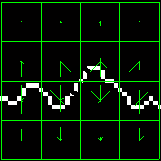
\includegraphics[width=6cm]{sampledescriptor.png}
\caption{The local patch is located around a sample point plotted on the temporary image. All the sample points are interpolated using the Bresenham algorithm. The 4x4 block grid can be seen on the patch as well as the green arrows showing the dominant gradient on each block.}
\label{fig:sampledescriptor}
\end{figure}


\subsubsection{Classification}

The classification is carried out by using a discriminative semi-supervised classification method, the Naive Bayes Nearest Neighbout (NBNN) \citep{Boiman2008} and the first step consists in extracting labelled descriptors from the training set for each class which are thus grouped together in two KD-tree \citep{Vedaldi2010} database structures.

%BCI Simulation vs k-fold cross validation.  It is quite known and understood that because the same experience will not generate the same markers in the EEG, BCI Simulation is sometimes better suited to understand how the device will operate on a real online application (the graeat variability of BCI).

While doing classification based on local features, which encode partial information, one problem that frequently arises is how to ensemble the individual classification of each local characteristic to the image that were used to derive those descriptors.

The NBNN algorithm tackles this problem by comparing each image against a whole classification class which is characterized by the set of descriptors that are closest to each one of the descriptors obtained for the query image.  The algorithm is based on \ref{eq:classification},

\begin{equation}
\hat{C} = argmin_C \sum_{}^{} \left\lVert d_i - NN_C(d_i) \right\rVert ^2
\label{eq:classification}
\end{equation}

\noindent where the predicted class $\hat{C}$ of a query image is calculated as the class $ C $ that minimize the summation of the $ L^2 $ distance between each descriptor $ d_i $ that belongs to the query image and its corresponding near neighbour $ NN_C(d_i) $ descriptor from each class.


\subsubsection{Parameters}

This method's parameters were selected according to the experimental protocol.  As the P300 event latency varies greatly between subjects, it is necessary to provide a descriptor that will be able to capture an entire transient event.  Equations \ref{eq:mapping1} and \ref{eq:mapping2} can be used to map the original signal parameters to local image patch structure. 

\begin{equation}
s = \frac{\Delta \mu V}{4 \cdot 3} \cdot \gamma 
\label{eq:mapping1}
\end{equation}

\begin{equation}
s = \frac{\lambda \cdot Fs}{4 \cdot 3} \cdot \gamma
\label{eq:mapping2}
\end{equation}

\noindent where $ Fs $ is the sample frequency of the EEG signal, $ \lambda $ is the length in seconds covered by the patch, and $ \mu V $ corresponds to the amplitude in microvolts that can be covered by the height of the patch.   By using $ s = 3 $ and a double scale of the image $ \gamma = 2 $ this gives the local patch, and the descriptor, the ability to identify events of 18 $ \mu V $ of amplitude of $ \lambda = 0.5 s $.  Finally, descriptors locations $ T $ were selected as suggested by the dataset publisher \citep{Riccio2013} between 0.2s and 0.7s after the onset of the stimulus. 

%\begin{figure}[H]
%\centering
%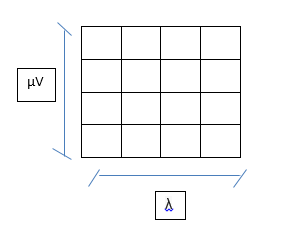
\includegraphics[width=16cm]{localpatch.png}
%\caption{The local patch is mapped to the original image by their correspondence .}
%\label{fig:sampledescriptor}
%\end{figure}

%%%%%%%%%%%%%%%%%%%%%%%%%%%%%%%%%%%%%%%%%%
\section{Results}
\label{section:results}
In Figure \ref{fig:subjectaveraged} the grand average (point-to-point) for all the subjects using the whole trial (i.e. 120 repetitions) is shown.  The P300 characteristic curve can be seen particularly in subjects 2, and 6 and in a lesser extend in the remaining subjects. In order to obtain a valid binary classification on averaged signals, particular care was observed to avoid unbalanced samples, because that may introduce a bias in the classification procedure (the variance of average signals is inversely proportional to the number of samples and the procedure would be discriminating signals with different variances). Especially in the case of the P300 response, the oddball paradigm requires that one of the stimuli need to be infrequent so that will unavoidably force the data to be unbalanced (i.e. an unequal number of trials in each condition) \citep{Tibon2015}.


\begin{figure}[H]
\centering

\includegraphics[width=16cm]{subjectaveraged.eps}
\caption{Point-To-Point grand averages of epochs obtained for hits (solid line) and no hits (dashed line) for each one of the 8 subjects for channel Cz. The P300 characteristic curve can be well identified particularly on subjects 2 and 6.}
\label{fig:subjectaveraged}
\end{figure}

Results are shown in Table \ref{tab:results} where BCI accuracy
for the Cz channel is calculated and compared with the values obtained by the publisher of the dataset  \citep{Riccio2013}.  Additionally the best performing channel is informed as well as its accuracy value.  It is of particular interest that using this method, the best performing channel was not always Cz, and instead occipital channels PO8 and PO7 showed very good performance indeed \citep{Huggins2016,Jure2016}.


\begin{table}[H]
\caption{Accuracy levels obtained by a 3-fold cross validation. The values reported by the dataset publishers for Cz are reproduced here for comparison. Additionally, BCI accuracies for channel Cz can be seen as well as performance levels and their standard deviation obtained for the BPC, the best performing channel for each subject.}
\centering
%% \tablesize{} %% You can specify the fontsize here, e.g.  \tablesize{\footnotesize}. If commented out \small will be used.
\begin{tabular}{ccccc}
\toprule
\textbf{Participant}	& \textbf{Original Cz}	& \textbf{ACC at Cz}	& \textbf{BPC}	& \textbf{Performance}\\
\midrule
1     &   0.84 &   0.79 & Cz  &   0.79 $\pm$ 0.01 \\
2     &   0.86 &   0.81 & PO7 &   0.93 $\pm$ 0.01 \\
3     &   0.87 &   0.78 & Cz  &   0.78 $\pm$ 0.03 \\
4     &   0.86 &   0.68 & PO8 &   0.90 $\pm$ 0.01 \\
5     &   0.86 &   0.80 & PO7 &   0.93 $\pm$ 0.01 \\
6     &   0.89 &   0.96 & Cz  &   0.96 $\pm$ 0.01 \\
7     &   0.89 &   0.78 & PO7 &   0.93 $\pm$ 0.01 \\
8     &   0.92 &   0.91 & PO7 &   1.00 $\pm$ 0.00 \\
\bottomrule
\end{tabular}
\label{tab:results}
\end{table}

The ITR, or BTR, in the case of reactive BCIs \citep{WolpawJonathanR2012} strongly depends on the amount of signal averaging required to transmit a valid and robust selection.  There is a trade-off that needs to be balanced between the required number of repetitions for each trial to guarantee robust transmission and the the achieved speed of transmission affected by the repetitions.  As detailed in the table \ref{tab:singletrialreduction} by applying this method, accuracy levels are only reduced in 20 percent even by using only one sequence of 12 repetitions (i.e. an entire flashing of the whole matrix).

\begin{table}[H]
\caption{Accuracy levels obtained by performing a BCI simulation on the testing dataset (4 letters). The BPC, best performing channel is shown and also performance levels for the 120, 60 and 12 repetitions. Finally the PR, performance reduction as a rate of reduction compared to the accuracy obtained using the entire trial, is described.  Almost all the subjects performed around 70\% even by averaging only 2 epochs for each class.}
\centering
%% \tablesize{} %% You can specify the fontsize here, e.g.  \tablesize{\footnotesize}. If commented out \small will be used.
\begin{tabular}{cccccc}
\toprule
\textbf{Participant}	& \textbf{BPC}	& \textbf{ACC@120}	& \textbf{ACC@60}	&  \textbf{ACC@12} & \textbf{PR}\\
\midrule
1 & Cz &   0.80 &   0.82 &   0.72 & 9\% \\
2 & PO7 &   0.93 &   0.78 &   0.75 & 18\%\\
3 & Cz &   0.80 &   0.82 &   0.72 & 9\%\\
4 & PO8 &   0.93 &   0.78 &   0.65 & 29\%\\
5 & PO7 &   0.93 &   0.78 &   0.75 & 18\%\\
6 & Cz &   0.80 &   0.82 &   0.72 & 9\%\\
7 & PO7 &   0.93 &   0.78 &   0.75 & 18\%\\
8 & PO7 &   0.93 &   0.78 &   0.75 & 18\%\\
\bottomrule
\end{tabular}
\label{tab:singletrialreduction}
\end{table}

%%%%%%%%%%%%%%%%%%%%%%%%%%%%%%%%%%%%%%%%%%
\section{Discussion}

This method, different from other methods which is based on the nonlinearity of the gradient of histograms which can be used to detect 

is also based on how the image look like.

SNR of p300 and how to detect it

Check if you can use this to detect any kind of transient signal.

Compare if it is possible with the descriptors from one subject, discriminate the others.

Channal identification based on the metric distance between the bags


%%%%%%%%%%%%%%%%%%%%%%%%%%%%%%%%%%%%%%%%%%
\section{Conclusion}

A method to characterize and classify EEG signals where the main characteristic can be both, rhythmic in nature as in motor imagery, and also transient in time space, like the P300 has been presented.

Although single trial classification was not perfectly achieved, it has been shown that this method could be applied with a P300 Speller Matrix application with increased ITR.

%Databases of descriptors.  Flexibility of the descriptor in terms of configuration and size (reference variants of SIFT on lower dimensiones).

The adaptive behaviour of the algorithm make it well suited when the shape of the pattern elicited by the P300 response, does not conform to the predicted structure.  This is due to the fact that the descriptors are directly based on how the signals actually looked like for the training and calibration step, and they do not require any prior knowledge about the signal.  This is of particular relevance for studies on outliers populations as may be the case for people who suffered some form of neuro-degenerative disorder like Lou Gehrig's disease.

The expanding of the understanding of this tool in order to automatically classify patterns in EEG, that are specifically identified by their shapes, is a prospect future work to be considered.  It may also provide  assistance to physician or electroencephalographers to help them locate these EEG patterns particularly in long recording periods \citep{Hartman2005}, frequent in sleep research.

Moreover, this method can be used as an alternate \textit{BCI predictor} \citep{Clerc} or as a tool for artefact removal (which is performed on many occasions by visually inspecting the signal).

%%%%%%%%%%%%%%%%%%%%%%%%%%%%%%%%%%%%%%%%%%
%\subsection{Subsection}
%
%\subsubsection{Subsubsection}
%
%Bulleted lists look like this:
%\begin{itemize}[leftmargin=*,labelsep=4mm]
%\item	First bullet
%\item	Second bullet
%\item	Third bullet
%\end{itemize}
%
%Numbered lists can be added as follows:
%\begin{enumerate}[leftmargin=*,labelsep=3mm]
%\item	First item
%\item	Second item
%\item	Third item
%\end{enumerate}
%
%The text continues here.



%%%%%%%%%%%%%%%%%%%%%%%%%%%%%%%%%%%%%%%%%%
\vspace{6pt} 

%%%%%%%%%%%%%%%%%%%%%%%%%%%%%%%%%%%%%%%%%%
%% optional
%\supplementary{The following are available online at www.mdpi.com/link, Figure S1: title, Table S1: title, Video S1: title.}

%%%%%%%%%%%%%%%%%%%%%%%%%%%%%%%%%%%%%%%%%%
\acknowledgments{This project was supported by the ITBACyT-15 funding program issued by ITBA University.}

%%%%%%%%%%%%%%%%%%%%%%%%%%%%%%%%%%%%%%%%%%
\authorcontributions{This projects is part of a the first author's PhD Thesis which is directed by Juan Miguel Santos and codirected by Ana Julia Villar.}

%%%%%%%%%%%%%%%%%%%%%%%%%%%%%%%%%%%%%%%%%%
\conflictofinterests{The authors declare no conflict of interest.} 

%%%%%%%%%%%%%%%%%%%%%%%%%%%%%%%%%%%%%%%%%%
%% optional
\abbreviations{The following abbreviations are used in this manuscript:\\

\noindent EEG: electroencephalography\\
BCI: Brain Computer Interfaces\\
SNR: Signal to Noise Ratio\\
CNS: Central Nervous System\\
ALS: Amyotrophic Lateral Sclerosis\\
ERP: Event-Related Potential\\
P300: Positive deflection of an Event-Related Potential which occurs 300 ms after onset of stimulus\\
ITR: Information Transfer Rate\\
BTR: Bit Transfer Rate\\
SIFT: Scale Invariant Feature Transform\\
HOG: Histogram Of Gradients}

%%%%%%%%%%%%%%%%%%%%%%%%%%%%%%%%%%%%%%%%%%
%% optional
%\appendixtitles{no} %Leave argument "no" if all appendix headings stay EMPTY (then no dot is printed after "Appendix A"). If the appendix sections contain a heading then change the argument to "yes".
%\appendixsections{multiple} %Leave argument "multiple" if there are multiple sections. Then a counter is printed ("Appendix A?). If there is only one appendix section then change the argument to ?one? and no counter is printed (?Appendix?).
%\appendix
%\section{}
%The appendix is an optional section that can contain details and data supplemental to the main text. For example, explanations of experimental details that would disrupt the flow of the main text, but nonetheless remain crucial to understanding and reproducing the research shown; figures of replicates for experiments of which representative data is shown in the main text can be added here if brief, or as Supplementary data. Mathemtaical proofs of results not central to the paper can be added as an appendix.
%
%\section{}
%All appendix sections must be cited in the main text. In the appendixes, Figures, Tables, etc. should be labeled starting with `A', e.g., Figure A1, Figure A2, etc. 

%%%%%%%%%%%%%%%%%%%%%%%%%%%%%%%%%%%%%%%%%%
% Citations and References in Supplementary files are permitted provided that they also appear in the reference list here. 
\bibliographystyle{mdpi}

%=====================================
% References, variant A: internal bibliography
%=====================================
%\renewcommand\bibname{References}
%\begin{thebibliography}{999}
% Reference 1
%\bibitem{ref-journal}
%Lastname, F.; Author, T. The title of the cited article. {\em Journal Abbreviation} {\bf 2008}, {\em 10}, 142-149.
% Reference 2
%\bibitem{ref-book}
%Lastname, F.F.; Author, T. The title of the cited contribution. In {\em The Book Title}; Editor, F., Meditor, A., Eds.; Publishing House: City, Country, 2007; pp. 32-58.
%\end{thebibliography}

%=====================================
% References, variant B: external bibliography
%=====================================
\bibliography{article}

%%%%%%%%%%%%%%%%%%%%%%%%%%%%%%%%%%%%%%%%%%
%% optional
%\sampleavailability{Samples of the compounds ...... are available from the authors.}

%%%%%%%%%%%%%%%%%%%%%%%%%%%%%%%%%%%%%%%%%%
\end{document}